%presentation about particle tracker using IGA

\documentclass[colorbacktitle,inverttitle,landscape,presentation,
	english,
	aspectratio=43, %43 or 169, 1610
	accentcolor=tud9b, %tud9b (temf) or tud5b (gsce) 
]{tudbeamer}

%%additional packages
%%language:
\usepackage[utf8]{inputenc}
\usepackage[english]{babel}
%%math:
\usepackage{amsmath}
\usepackage{mathtools}
%%tikz:
\usepackage{tikz}
\usetikzlibrary{patterns}
\usepackage[siunitx,americaninductors]{circuitikz}
\usepackage{siunitx}
%%pgfplots:
\usepackage{pgfplots}
\usepgfplotslibrary{groupplots}
\usepgfplotslibrary{patchplots}
\usepackage{pgfplotstable}
\pgfplotsset{compat=newest}\usepgfplotslibrary{units}
%%scaling:
\usepackage{adjustbox}
%%temf macros:
%\let\Laplace\zz % workaround since clash with trfsigns
%\usepackage{temf-names}
%\let\zz\Laplace		%Ausgeklammert 17.4. f V1
%\usepackage{temf-finite}
%\usepackage{temf-fields}
%\usepackage{temf-matrixvector}
%\usepackage{notInTemfMacros}
%needs to come last
\usepackage{temfbeamer}

%remove TU logo from every slide but the title
\setbeamertemplate{headline}[TUD theme nologo] 

%set date
\date{May 30, 2018}

%%%%%%%%%%%%%%%%%%%%%%%%%%%%%%%%%%%%%%%%%%%%%%%%%%%%%%%%%%%%%%%%%%%%%%%%%%%%%%%%%%%%%%%%%%%%%%%%%%%%%%%%%%%%%%%%%%%%%%%%%%%%%%%%%%%%%%

\title{Particle Tracking using Isogeometric Analysis}

\subtitle{\\[0.3\baselineskip]
	Peter Förster\\[0.3\baselineskip]
{\small Jacopo Corno, M.Sc. and Prof. Dr. Sebastian Schöps}\\
[0.3\baselineskip]
{\tiny Proseminar ETiT}\\[0.3em]
	\mbox{\scriptsize}~}
	
\institute[TU Darmstadt | Fachbereich 18 | Institut Theorie Elektromagnetischer Felder]{Institut für Theorie Elektromagnetischer Felder, TU Darmstadt}

%%%%%%%%%%%%%%%%%%%%%%%%%%%%%%%%%%%%%%%%%%%%%%%%%%%%%%%%%%%%%%%%%%%%%%%%%%%%%%%%%%%%%%%%%%%%%%%%%%%%%%%%%%%%%%%%%%%%%%%%%%%%%%%%%%%%%%

\begin{document}
	
\begin{titleframe}
	\tudtitle[images/temf_logo.pdf]{images/temf_background.jpg} 
	%\tudtitle[images/gsce_logo.pdf]{images/gsce_background.jpg}
	\end{titleframe}
	
\begin{frame}
	\frametitle{Outline}
	\tableofcontents%[currentsection,subsectionstyle=show/show/hide]
\end{frame}
	
%%%%%%%%%%%%%%%%%%%%%%%%%%%%%%%%%%%%%%%%%%%%%%%%%%%%%%%%%%%%%%%%%%%%%%%%%%%%%%%%%%%%%%%%%%%%%%%%%%%%%%%%%%%%%%%%%%%%%%%%%%%%%%%%%%%%%%
	
\section{Motivation}
\begin{frame}
\frametitle{Motivation}
	\begin{itemize}
	\item analysis of the beam inside an accelerator is crucial during development
	
	\item particle tracker can be used to provide a simulation of the beam characteristics
	
	\item results can be used to optimize the geometry of the accelerator
	\end{itemize}
\end{frame}

\begin{frame}
\frametitle{Problem Setting}
	\begin{itemize}
	\item the electric and magnetic field inside the accelerator need to be computed/determined 
	
	\item electric field is calculated by solving Poisson's equation for the electrostatic potential
	
	\item complex geometries with curved parts are better approximated using IGA then e.g. FEM or FIT
	
	\item model equations describing the particle motions need to be solved
	\end{itemize}
\end{frame}
		
%%%%%%%%%%%%%%%%%%%%%%%%%%%%%%%%%%%%%%%%%%%%%%%%%%%%%%%%%%%%%%%%%%%%%%%%%%%%%%%%%%%%%%%%%%%%%%%%%%%%%%%%%%%%%%%%%%%%%%%%%%%%%%%%%%%%%%

\section{Problem setting}
%\begin{frame}
%\frametitle{Mathematical model}
%	\begin{itemize}
%	\item the model equations read
%	\begin{equation*}
%	\frac{\d\rmat_i}{\d t} = \vmat_i\\
%	\frac{\d m_e\vmat_i}{\d t} = e(\Emat + \vmat_i\times\Bmat)\\
%	i = 1\dots N
%	\end{equation*}
%	where $e$ is the electron charge, $m_e$ is the relativistic electron mass; $\rmat_i$ and $\vmat_i$ denote particle positions and velocities respectively
%	
%	\item only taking into account electrostatic particle-particle interactions the space-charge field $\Emat$ is determinded by
%	\begin{equation*}
%\nabla(\eps\Emat) = \frac{1}{\eps_0}\sum_i^N q_i \delta(\rmat-\rmat_i),\ \Emat = -\nabla \phifield,
%	\end{equation*}
%	where $\eps$ is the permittivity and $q_i$ the charge of the $i$-th particle	
%	\end{itemize}
%\end{frame}

%\begin{frame}
%\frametitle{Space Charge Limited Emission}
%	\begin{itemize}
%	\item the Child-Langmuir diode equation reads
%	\begin{equation*}
%	J_\mathrm{CL} = \right(\frac{4\eps_0}{9}\left)\sqrt{\frac{2e}{m_e}}\frac{\delta\phifield_b^{3/2}}{\delta d^2},
%	\end{equation*}
%	where $J_\mathrm{CL}$ is the current at the emission surface and $\delta\phifield_b$ the local potential difference at a distance $\delta d$ from the surface		
%\end{frame}

%%%%%%%%%%%%%%%%%%%%%%%%%%%%%%%%%%%%%%%%%%%%%%%%%%%%%%%%%%%%%%%%%%%%%%%%%%%%%%%%%%%%%%%%%%%%%%%%%%%%%%%%%%%%%%%%%%%%%%%%%%%%%%%%%%%%%%

\section{Validation of WR}
\begin{frame}
\frametitle{Validation of WR}	
	\begin{itemize}
	\item MQS device represents a steel pipe cross section
		
	\item aim is to calculate the magnetic flux density inside the MQS device
	
	\item monolithic solution (Mono) is used as reference
	\end{itemize}		
	
	\begin{figure}
	\begin{minipage}{0.5\textwidth}
	\begin{center}
	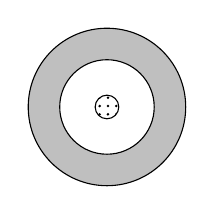
\begin{tikzpicture}[scale = 0.5]
	\filldraw[fill=lightgray, draw=black] (0,0) circle[radius=2];
	\filldraw[fill=white, draw=black] (0,0) circle[radius=1.2];
	\draw[pattern=dots, pattern color=black] (0,0) circle[radius=0.3];
	\end{tikzpicture}
	\caption{steel pipe cross section}
	\end{center}
	\end{minipage}\begin{minipage}{0.5\textwidth}
	\begin{center}
	\begin{adjustbox}{scale=0.4}
	\begin{circuitikz}
	\draw (0,0)
	to[sV,v=$v_s$] (0,2)
	to[R=$R_S$] (2,2)
	to[L=$L_S$] (4,2)
	to[C=$C_S$] (6,2)
	to[short] (6,2)
	to[R=$R_P$] (6,0);
	\draw (6,2)
	to[short] (8,2) 
	to[L=$L_P$] (8,0);
	\draw (8,2)
	to[short] (10,2)
	to[C=$C_P$] (10,0);
	\draw (10,2)
	to[short] (12,2)
	to[twoport, t=$MQS$] (12,0)
	to[short] (0,0);	
	\end{circuitikz}
	\end{adjustbox}
	\caption{circuit with MQS device}
	\end{center}
	\end{minipage}
	\end{figure}
\end{frame}

\begin{frame}
\frametitle{Validation of WR}
%	\begin{figure}
%	\begin{minipage}{0.5\textwidth}
%	\begin{center}
%	\begin{tikzpicture}[scale=0.6]
%		\begin{semilogyaxis}[
%		xlabel={$k$-th iteration},
%		ylabel={$\frac{\| \mathbf{i}_n^{(k)} - \mathbf{i}_n^{(k-1)}\|_2}{\| \mathbf{i}_n^{(k)}\|_2}$},
%		grid=major,
%		cycle multi list={color list\nextlist [1 of]mark list},
%		legend entries={$T_0$, $T_1$, $T_2$}]
%		\addplot table[x=k, y=diff, col sep=comma] {images/WR_small_window_size/diff_1_WR_small_window_size.csv};
%		\addplot table[x=k, y=diff, col sep=comma] {images/WR_small_window_size/diff_2_WR_small_window_size.csv};
%		\addplot table[x=k, y=diff, col sep=comma] {images/WR_small_window_size/diff_3_WR_small_window_size.csv};
%		\end{semilogyaxis}
%	\end{tikzpicture}
%	\caption{convergence of WR for small time windows}
%	\end{center}
%	\end{minipage}\begin{minipage}{0.5\textwidth}
%	\begin{center}
%	\begin{tikzpicture}[scale=0.6]
%		\begin{semilogyaxis}[
%		xlabel={$k$-th iteration},
%		ylabel={$\frac{\| \mathbf{i}_n^{(k)} - \mathbf{i}_n^{(k-1)}\|_2}{\| \mathbf{i}_n^{(k)}\|_2}$},
%		grid=major,
%		cycle multi list={color list\nextlist [1 of]mark list},
%		legend entries={$T_0$, $T_1$, $T_2$}]
%		\addplot table[x=k, y=diff, col sep=comma] {images/WR_large_window_size/diff_1_WR_large_window_size.csv};
%		\addplot table[x=k, y=diff, col sep=comma] {images/WR_large_window_size/diff_2_WR_large_window_size.csv};
%		\addplot table[x=k, y=diff, col sep=comma] {images/WR_large_window_size/diff_3_WR_large_window_size.csv};
%		\end{semilogyaxis}
%	\end{tikzpicture}
%	\caption{convergence of WR for large time windows}
%	\end{center}
%	\end{minipage}
%	\end{figure}
\end{frame}

%%%%%%%%%%%%%%%%%%%%%%%%%%%%%%%%%%%%%%%%%%%%%%%%%%%%%%%%%%%%%%%%%%%%%%%%%%%%%%%%%%%%%%%%%%%%%%%%%%%%%%%%%%%%%%%%%%%%%%%%%%%%%%%%%%%%%%

\section{Parareal algorithm}
\begin{frame}
\frametitle{Parareal algorithm}
	\begin{itemize}
	\item uses a very accurate and costly fine propagator, computed in parallel
	
	\item uses a less accurate but cheap coarse propagator, computed sequentially
	\end{itemize}
	
	\begin{figure}
	\begin{minipage}{0.5\textwidth}
	\begin{center}
	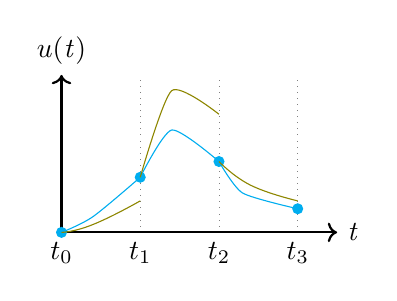
\begin{tikzpicture}[scale=1]
	\draw[dotted,very thin,gray] (1,0) -- (1,2);
	\draw[dotted,very thin,gray] (2,0) -- (2,2);
	\draw[dotted,very thin,gray] (3,0) -- (3,2);
	\draw [<->,thick] (0,2) node (yaxis) [above] {$u(\mathit{t})$} |- (3.5,0) node (xaxis) [right] {$\mathit{t}$};
	\draw (0,0) node[below]{\textcolor{black}{$t_{0}$}};
	\draw (1,0) node[below]{\textcolor{black}{$t_{1}$}};
	\draw (2,0) node[below]{\textcolor{black}{$t_{2}$}};
	\draw (3,0) node[below]{\textcolor{black}{$t_{3}$}};
	\coordinate (A) at (0,0) {};
	\coordinate (B) at (1,0.7) {};
	\coordinate (C) at (2,0.9) {};
	\coordinate (D) at (3,0.3) {};
	\fill [cyan] (A) circle(2pt);
	\draw [cyan] plot [smooth, tension=0.5] coordinates{(A) (0.4,0.2) (B)};
	\fill [cyan] (B) circle(2pt);
	\draw [cyan] plot [smooth, tension=0.4] coordinates{(B) (1.4,1.3) (C)};
	\fill [cyan] (C) circle(2pt);
	\draw [cyan] plot [smooth, tension=0.4] coordinates{(C) (2.3,0.5) (D)};
	\fill [cyan] (D) circle(2pt);
	\coordinate (E) at (1,0.4) {};
	\coordinate (F) at (2,1.5) {};
	\coordinate (G) at (3,0.4) {};
	\draw [olive] plot [smooth, tension=0.9] coordinates{(A) (0.4,0.1) (E)};
	\draw [olive] plot [smooth, tension=0.4] coordinates{(B) (1.4,1.8) (F)};
	\draw [olive] plot [smooth, tension=0.8] coordinates{(C) (2.4,0.6) (G)};
	\end{tikzpicture}
	\caption{first iteration of coarse propagator in \textcolor{cyan}{cyan} and fine propagator in \textcolor{olive}{olive}, initial values for fine marked in \textcolor{cyan}{cyan}}
	\end{center}
	\end{minipage}\begin{minipage}{0.5\textwidth}
	\begin{center}
	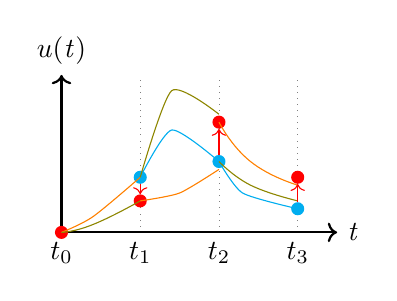
\begin{tikzpicture}[scale=1,node distance=2cm]
	\draw[dotted,very thin,gray] (1,0) -- (1,2);
	\draw[dotted,very thin,gray] (2,0) -- (2,2);
	\draw[dotted,very thin,gray] (3,0) -- (3,2);
	\draw [<->,thick] (0,2) node (yaxis) [above] {$u(\mathit{t})$} |- (3.5,0) node (xaxis) [right] {$\mathit{t}$};
	\draw (0,0) node[below]{\textcolor{black}{$t_{0}$}};
	\draw (1,0) node[below]{\textcolor{black}{$t_{1}$}};
	\draw (2,0) node[below]{\textcolor{black}{$t_{2}$}};
	\draw (3,0) node[below]{\textcolor{black}{$t_{3}$}};
	\node [fill,circle,red,scale=0.5] (A) at (0,0) {};
	\node [fill,circle,cyan,scale=0.5] (B) at (1,0.7) {};
	\node [fill,circle,cyan,scale=0.5] (C) at (2,0.9) {};
	\node [fill,circle,cyan,scale=0.5] (D) at (3,0.3) {};
	\draw [orange] plot [smooth, tension=0.5] coordinates{(A) (0.4,0.2) (B)};
	\draw [cyan] plot [smooth, tension=0.4] coordinates{(B) (1.4,1.3) (C)};
	\draw [cyan] plot [smooth, tension=0.4] coordinates{(C) (2.3,0.5) (D)};
	\node [fill,circle,red,scale=0.5] (E) at (1,0.4) {};
	\draw [->,red] (B) -- (E);
	\coordinate (F) at (2,1.5) {};
	\coordinate (G) at (3,0.4) {};
	\draw [olive] plot [smooth, tension=0.9] coordinates{(A) (0.4,0.1) (E)};
	\draw [olive] plot [smooth, tension=0.4] coordinates{(B) (1.4,1.8) (F)};
	\draw [olive] plot [smooth, tension=0.8] coordinates{(C) (2.4,0.6) (G)};
	\coordinate (H) at (2,0.8);
	\coordinate (I) at (3,0.6);
	\node [fill,circle,red,scale=0.5] (K) at (2,1.4) {};
	\draw [->,red] (C) -- (K);
	\draw [orange] plot [smooth, tension=0.4] coordinates{(E) (1.5,0.5) (H)};
	\draw [orange] plot [smooth, tension=0.9] coordinates{(K) (2.4,0.9) (I)};
	\node [fill,circle,red,scale=0.5] (L) at (3,0.7) {};
	\draw [->,red] (D) -- (L);	
	\end{tikzpicture}
	\caption{second iteration of coarse propagator in \textcolor{orange}{orange}, updated initial values in \textcolor{red}{red}}
	\end{center}
	\end{minipage}
	\end{figure}
\end{frame}

%%%%%%%%%%%%%%%%%%%%%%%%%%%%%%%%%%%%%%%%%%%%%%%%%%%%%%%%%%%%%%%%%%%%%%%%%%%%%%%%%%%%%%%%%%%%%%%%%%%%%%%%%%%%%%%%%%%%%%%%%%%%%%%%%%%%%%

\section{Numerical Tests}
\begin{frame}

\end{frame}

%%%%%%%%%%%%%%%%%%%%%%%%%%%%%%%%%%%%%%%%%%%%%%%%%%%%%%%%%%%%%%%%%%%%%%%%%%%%%%%%%%%%%%%%%%%%%%%%%%%%%%%%%%%%%%%%%%%%%%%%%%%%%%%%%%%%%%

\begin{frame}
\frametitle{Conclusion}
	\begin{itemize}
	\item speedup is shown for different combinations of WR and PR
	
	\item \textit{(PR-WR)} provides speedup under many circumstances
	
	speedup for other variants depends on window size, among other factors
	
	\item all combinations of WR and PR maintain the benefits of WR
	\end{itemize}
\end{frame}

%%%%%%%%%%%%%%%%%%%%%%%%%%%%%%%%%%%%%%%%%%%%%%%%%%%%%%%%%%%%%%%%%%%%%%%%%%%%%%%%%%%%%%%%%%%%%%%%%%%%%%%%%%%%%%%%%%%%%%%%%%%%%%%%%%%%%%

\begin{frame}
\frametitle{List of References}
	\begin{enumerate}
	\item[{[1]}]
Sebastian Schöps, Idoia Cortes Garcia, Michał Maciejewski and Bernhard
Auchmann. Reduced Order Modelling for the Simulation of Quenches in
Superconducting Magnets. In Proceedings of the 7th GACM Colloquium on
Computational Mechanics for Young Scientists from Academia and Industry
October 11-13, 2017 in Stuttgart, Germany.

	\item[{[2]}]
Sebastian Schöps, Herbert De Gersem, Thomas Weiland, (2013) "Winding
functions in transient magnetoquasistatic field-circuit coupled simulations",
COMPEL: The International Journal for Computation and Mathematics in
Electrical and Electronic Engineering, Vol. 32 Issue: 6, pp.2063-2083.

	\item[{[3]}]
Sebastian Schöps, Herbert De Gersem and Andreas Bartel. A
Cosimulation Framework for Multirate Time Integration of Field/Circuit
Coupled Problems. IEEE TRANSACTIONS ON MAGNETICS, VOL. 46,
NO. 8, pp.3233-3236, AUGUST 2010.
	\end{enumerate}
\end{frame}

\begin{frame}
\frametitle{List of References}
	\begin{enumerate}
	\item[{[4]}]
Jacques-Louis Lions, Yvon Maday, Gabriel Turinici. Résolution d’EDP par
un schéma en temps «pararéel». C. R. Acad. Sci. Paris, t. 332, Série I, p.
661–668, 2001.

	\item[{[5]}]
Thomas Cadeau and Frédéric Magoulès. Coupling the Parareal algorithm
with the Waveform Relaxation method for the solution of Differential
Algebraic Equations. In Proceedings of the 10th International Symposium
on Distributed Computing and Applications to Business, Engineering and
Science. 2011.

	\item[{[6]}]
Chung-Wen Ho, Albert E. Ruehli and Pierce A. Brennan. The Modified
Nodal Approach to Network Analysis. IEEE Transactions on Circuits and Systems, Vol. 22, No.6, pp.504-509, June 1975.
	\end{enumerate}
\end{frame}
	
	
\end{document}